%  LaTeX support: latex@mdpi.com 
%  For support, please attach all files needed for compiling as well as the log file, and specify your operating system, LaTeX version, and LaTeX editor.

%=================================================================
\documentclass[entropy,article,submit,pdftex,moreauthors]{Definitions/mdpi} 

%=================================================================
% MDPI internal commands - do not modify
\firstpage{1} 
\makeatletter 
\setcounter{page}{\@firstpage} 
\makeatother
\pubvolume{1}
\issuenum{1}
\articlenumber{0}
\pubyear{2024}
\copyrightyear{2024}
%\externaleditor{Academic Editor: Firstname Lastname}
\datereceived{ } 
\daterevised{ } % Comment out if no revised date
\dateaccepted{ } 
\datepublished{ } 
%\datecorrected{} % For corrected papers: "Corrected: XXX" date in the original paper.
%\dateretracted{} % For corrected papers: "Retracted: XXX" date in the original paper.
\hreflink{https://doi.org/} % If needed use \linebreak
%\doinum{}
%\pdfoutput=1 % Uncommented for upload to arXiv.org
%\CorrStatement{yes}  % For updates


%=================================================================
% Add packages and commands here. The following packages are loaded in our class file: fontenc, inputenc, calc, indentfirst, fancyhdr, graphicx, epstopdf, lastpage, ifthen, float, amsmath, amssymb, lineno, setspace, enumitem, mathpazo, booktabs, titlesec, etoolbox, tabto, xcolor, colortbl, soul, multirow, microtype, tikz, totcount, changepage, attrib, upgreek, array, tabularx, pbox, ragged2e, tocloft, marginnote, marginfix, enotez, amsthm, natbib, hyperref, cleveref, scrextend, url, geometry, newfloat, caption, draftwatermark, seqsplit
% cleveref: load \crefname definitions after \begin{document}

%=================================================================
% Please use the following mathematics environments: Theorem, Lemma, Corollary, Proposition, Characterization, Property, Problem, Example, ExamplesandDefinitions, Hypothesis, Remark, Definition, Notation, Assumption
%% For proofs, please use the proof environment (the amsthm package is loaded by the MDPI class).

%=================================================================
% Full title of the paper (Capitalized)
\Title{How Information Evolves}

% MDPI internal command: Title for citation in the left column
\TitleCitation{How Information Evolves}

% Authors, for the paper (add full first names)
\Author{Dan Adler $^{1}$}

%\longauthorlist{no}

% MDPI internal command: Authors, for metadata in PDF
\AuthorNames{Dan Adler}

% MDPI internal command: Authors, for citation in the left column
\AuthorCitation{Dan Adler}
% If this is a Chicago style journal: Lastname, Firstname, Firstname Lastname, and Firstname Lastname.

% Affiliations / Addresses (Add [1] after \address if there is only one affiliation.)
\address{%
$^{1}$ \quad dan@danadler.com}

%\simplesumm{} % Simple summary

%\conference{} % An extended version of a conference paper

% Abstract (Do not insert blank lines, i.e. \\) 
\abstract{The emergence of complexity and information is a fundamental question spanning disciplines from physics to biology and computation. While traditional approaches describe information as a static entity or rely on predefined mechanisms, they often leave unresolved how complexity arises dynamically from purely abiotic processes. This paper presents ABC systems, an abstract framework that models the evolution of patterns through probabilistic interactions and stability-driven selection. By abstracting away specific physical laws, these systems demonstrate a universal mechanism for generating order and information. ABC systems evolve patterns over successive generations, with selection pressures favoring stable configurations that persist and interact more frequently. These dynamics encode logic, computational rules, and even self-replicating behaviors, providing insights into the transition from abiotic processes to biotic evolution. The framework also highlights the interplay between top-down and bottom-up causality, illustrating how emergent patterns recursively influence their formation while being shaped by local interactions. This study offers a computationally realizable pathway to bridge randomness and complexity. It connects entropy reduction, emergent computation, and dynamic information storage, revealing a route for systems to transition from disordered states to ordered, low-entropy configurations capable of encoding and processing information.
}

% Keywords
\keyword{Abiotic evolution; Emergent complexity; Information dynamics; Stability-driven selection; Top-down causality; Bottom-up causality; Cellular automata; Bayesian updating; Entropy reduction; Probabilistic interactions; Computational emergence; Prebiotic systems}


\graphicspath{{images/}}

%%%%%%%%%%%%%%%%%%%%%%%%%%%%%%%%%%%%%%%%%%
\begin{document}
%%%%%%%%%%%%%%%%%%%%%%%%%%%%%%%%%%%%%%%%%%

% The order of the section titles is different for some journals. Please refer to the "Instructions for Authors” on the journal homepage.

\section{Introduction}

The study of evolution, complexity, and information has long been a cornerstone of multiple scientific disciplines, bridging physics, biology, and computation. Foundational works such as Schrödinger's \textit{What is Life?} \cite{schrodinger1944life} posed fundamental questions about how order emerges from disorder, inspiring theoretical explorations of how physical laws govern the emergence of biological systems. Similarly, Tegmark's \textit{Mathematical Universe Hypothesis} \cite{tegmark2008mathematical} posits that the universe itself is a mathematical structure, where physical phenomena are manifestations of abstract mathematical rules. These works frame the question of complexity but often leave the detailed mechanisms of emergence unaddressed.

In the realm of evolutionary dynamics, Nowak's seminal text \textit{Evolutionary Dynamics} \cite{nowak2006evolutionary} provides rigorous mathematical models that describe the mechanisms of replication, mutation, and selection. While these models illuminate the principles of biological evolution, they assume the existence of self-replicating entities and do not delve into how such entities might arise from purely abiotic processes. Similarly, Wheeler's concept of "It from Bit" \cite{wheeler1990itbit} intriguingly suggests that information underpins the physical world, but it lacks a concrete mechanism for how information structures form and evolve.

Dennis Noble's work on top-down causality \cite{noble2012causality} emphasizes the role of systems-level behavior in determining lower-level interactions. This perspective challenges reductionist paradigms but does not address how such systems might emerge from simpler, abiotic conditions. On the computational side, Seth Lloyd’s concept of the universe as a quantum computer \cite{lloyd2006programming} provides a framework for understanding the universe as a computational entity but leaves open the question of how specific computational rules or patterns arise.

Algorithmic complexity \cite{kolmogorov1965complexity} \cite{chaitin1977algorithmic} \cite{solomonoff1964formal} and Shannon’s information theory \cite{shannon1948mathematical} provide powerful tools for quantifying information and complexity but do not explain how information is created or evolves within physical systems. These frameworks focus on static measures of complexity, often missing the dynamic interplay between interactions and selection that drives the formation of ordered structures.

The approach proposed in this paper distinguishes itself by focusing on ABC systems, which offer an explicit, abstract model for the emergence of complexity and information. Unlike prior work that remains tied to specific physical systems or abstract concepts without implementation pathways, ABC systems provide a mechanism for how stable patterns arise, evolve, and persist based solely on probabilistic interactions and stability constraints. By abstracting out the specific physics of the system, ABC systems offer a universal framework applicable to a wide range of phenomena, from chemical interactions to computational models.

In contrast to Wheeler’s "It from Bit," which lacks a generative mechanism, ABC systems demonstrate how information structures emerge dynamically through selection pressures. Unlike evolutionary dynamics as formulated by Nowak, which assumes pre-existing replicators, ABC systems show how stable, self-replicating patterns can arise from purely abiotic interactions. Furthermore, the framework of ABC systems provides a path to connect the abstract ideas of Lloyd and Tegmark with practical, realizable dynamics, where probabilistic interactions evolve into ordered patterns encoding information.

This paper advances the field by demonstrating how the principles of stability-driven selection, feedback, and interaction probabilities can generate complexity and information in a way that bridges abiotic and biotic systems. By providing a detailed mechanism for the emergence of order, this work extends prior theories into a practical and computationally realizable framework.


\section{ABC System Fundamentals}

This paper considers "ABC Systems" defined as follows: a population of elements \( A, B, C, \dots \) capable of forming compounds through local interactions of unspecified forces. These elements could exist in our physical universe, or in an abstract universe. The stability of compounds determines how many generations they will persist, and we assume the base elements regenerate. Over successive generations, the system undergoes a form of natural selection where compound stability drives the evolution of the population. ABC systems are governed by two distinct but interrelated probability distributions: The population distribution, reflecting the relative abundance of patterns in the system, and the stability distribution, representing the likelihood that interactions between patterns are successful and result in new, stable patterns. Together, these distributions determine the dynamics of the system, including the selection of stable patterns, their evolution over generations, and the emergent information encoded within the system.

Consider a population of 3 elements: {A, B, C}. Assume B-compounds are more stable than those without B. Thus AB, BC, ABC, have a higher stability than AC or A or C. Therefore, B-compounds will persist over multiple generations, while the others will quickly dissipate. The more stable B-compounds will interact more frequently due to their relative frequency, even without replication or inheritance. A simulation may look like this:

\begin{figure}[htp]
    \centering
    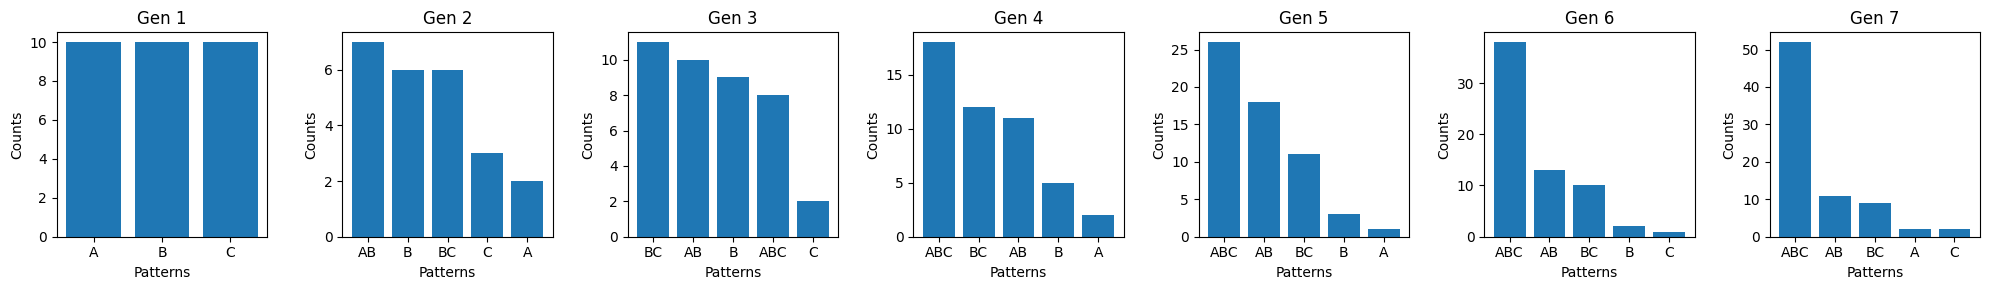
\includegraphics[width=13cm]{pat_1}
    \caption{ABC System population evolution simulation}
    \label{fig:pat_1}
\end{figure}

Where is Maxwell's demon \cite{leff2002maxwell} hiding in this example, driving it towards a low-entropy state? The answer lies in the roulette wheel. Compounds that persist longer have more chances to interact. As their frequency in the population grows, their chances to interact grow even more. In Evolutionary Dynamics, this is called fitness-proportionate selection \cite{back1996evolutionary} or roulette wheel selection \cite{goldberg1989genetic} \cite{holland1975adaptation}.

\section{Dual Probability Distributions Governing ABC Systems}

ABC systems can be effectively described by two interdependent probability distributions: the \textbf{population distribution}, which represents the relative abundance of patterns in the system, and the \textbf{stability distribution}, which quantifies the likelihood of successful interactions between patterns and the resulting stability of those interactions. These distributions interact to drive the system's dynamics, determining which patterns persist, dominate, or dissipate over time.

The population distribution reflects the probabilities of patterns at any given generation \( t \). Let \( P(p_t) \) represent the probability of pattern \( p \) in the population at time \( t \):
\[
P(p_t) = \frac{N(p_t)}{\sum_{q \in P} N(q_t)},
\]
where \( N(p_t) \) is the absolute count of pattern \( p \) in the population at time \( t \), and \( \sum_{q \in P} N(q_t) \) is the total population size at time \( t \), ensuring normalization (\( \sum_{p \in P} P(p_t) = 1 \)). The population distribution evolves over generations as patterns interact and new stable configurations emerge. As patterns with higher stability and frequent interactions become more prominent in the population, the population distribution evolves to reflects the history of past interactions and selection pressures.

The stability distribution represents the likelihood of successful interactions between patterns \( p \) and \( q \). Let \( S(p, q) \) denote the stability of the interaction between \( p \) and \( q \), defined as:
\[
S(p, q) = P(r | p, q),
\]
where \( P(r | p, q) \) is the conditional probability of forming pattern \( r \) as a result of the interaction between \( p \) and \( q \).

Stability reflects inherent properties of the patterns such as physical proximity, strength of bonds, geometric compatibility, energy barriers, or interaction rules. Stability values vary for different pairs of patterns, influencing which interactions dominate the dynamics. While the population distribution evolves rapidly, the stability distribution remains constant or changes only gradually.

\subsection{Combined Role of Population and Stability Distributions}

The two distributions together govern the dynamics of the system. The probability of two patterns \( p \) and \( q \) interacting to form a new pattern \( r \) is proportional to their population probabilities and the stability of their interaction:
\[
P(p_{t+1}) \propto P(p_t) \cdot \sum_{q \in P} P(q_t) \cdot S(p, q).
\]
The continuous-time dynamics of the feedback system can be derived as a natural extension of the discrete update equation:
\[
\frac{dP(p, t)}{dt} \approx \alpha P(p, t) \cdot S_{\text{eff}},
\]
where \( S_{\text{eff}} = \sum_{q \in P} P(q, t) \cdot S(p, q) \) is the effective stability of the pattern. Order is generated in the system through feedback-driven amplification of stable patterns. The probability of a pattern \( P(p, t) \) grows exponentially over time as a result of stabilizing interactions, following:
\[
P(p, t) \propto \exp(\alpha S_{\text{eff}} t),
\]
where \( \alpha \) is the growth rate constant, and \( S_{\text{eff}} \) is the effective stability of the pattern. This exponential growth rapidly increases the dominance of stable patterns in the population.

In contrast, random processes and stochastic fluctuations redistribute probabilities in the system, contributing to an increase in entropy. The degradation of order due to these random effects is characterized by a slower logarithmic growth in entropy:
\[
\Delta H \propto \ln(t).
\]
As time progresses, the competition between the exponential growth of stable patterns and the logarithmic increase in entropy becomes evident. The net result is that the exponential growth of order, driven by stabilizing feedback and represented as \( \exp(\alpha S_{\text{eff}} t) \), outpaces the entropy increase \( \ln(t) \). This ensures that stability-driven feedback creates a net reduction in entropy, leading the system toward a more ordered, low-entropy state. Over time, the dominance of stable patterns suppresses randomness, driving the system into configurations characterized by emergent complexity and order.

This analysis demonstrates how stability-driven interactions in local populations generate order faster than the second law of thermodynamics can degrade it. While random fluctuations tend to increase entropy, the exponential reinforcement of stable patterns creates a net reduction in entropy, leading to emergent order. The dynamics also highlight the competitive nature of the system: only patterns with sufficiently high stability and effective interaction networks survive over the long term, ensuring the self-organization of the population into ordered configurations.

\subsection{Catalysis}

Consider an ABC system where \( A \) interacts with \( B \) to form a compound \( AB \), but this interaction occurs only in the presence of a catalyst \( C \). The catalyst \( C \) is not consumed or altered during the interaction, yet it influences the system's dynamics by facilitating specific reactions. This creates selection pressure for \( C \) to persist due to its role in enabling the formation of stable compounds. In this case, the catalyst \( C \) facilitates the reaction by increasing its likelihood:
\[
P(A + B \to AB \mid C) \propto p_A \cdot p_B \cdot p_C.
\]

The catalyst \( C \) benefits indirectly, as its presence enables reactions that increase the overall fitness of the system.

\section{Mixing Two ABC Systems: Entropy Dynamics}

Mixing two independently evolved ABC systems introduces a new dimension to their dynamics, where patterns and interactions from each system influence the other. This interaction results in the exchange of information, changes in entropy, and the potential emergence of novel patterns. By analyzing information flow and entropy in such mixed systems, we can gain deeper insights into the dynamics of evolving systems and their capacity for self-organization.

\subsection{Setup for Mixing Two ABC Systems}

Let two independently evolved ABC systems \( P_1 \) and \( P_2 \) represent populations of patterns \( \{A, B, C, \dots\} \) and \( \{X, Y, Z, \dots\} \), respectively. Each system evolves independently based on its population distribution \( P(p_t) \) and stability constraints \( S(p, q) \) for patterns \( p, q \) within the same system.

When the two systems are mixed, the patterns from \( P_1 \) and \( P_2 \) interact, allowing the formation of cross-system compounds (e.g., \( ABX, XYZ \)). Stability constraints extend to cross-system interactions, introducing new terms \( S(p, q) \) where \( p \in P_1 \) and \( q \in P_2 \). The joint system evolves based on updated probabilities reflecting both within-system and cross-system interactions.

\begin{figure}[htp]
    \centering
    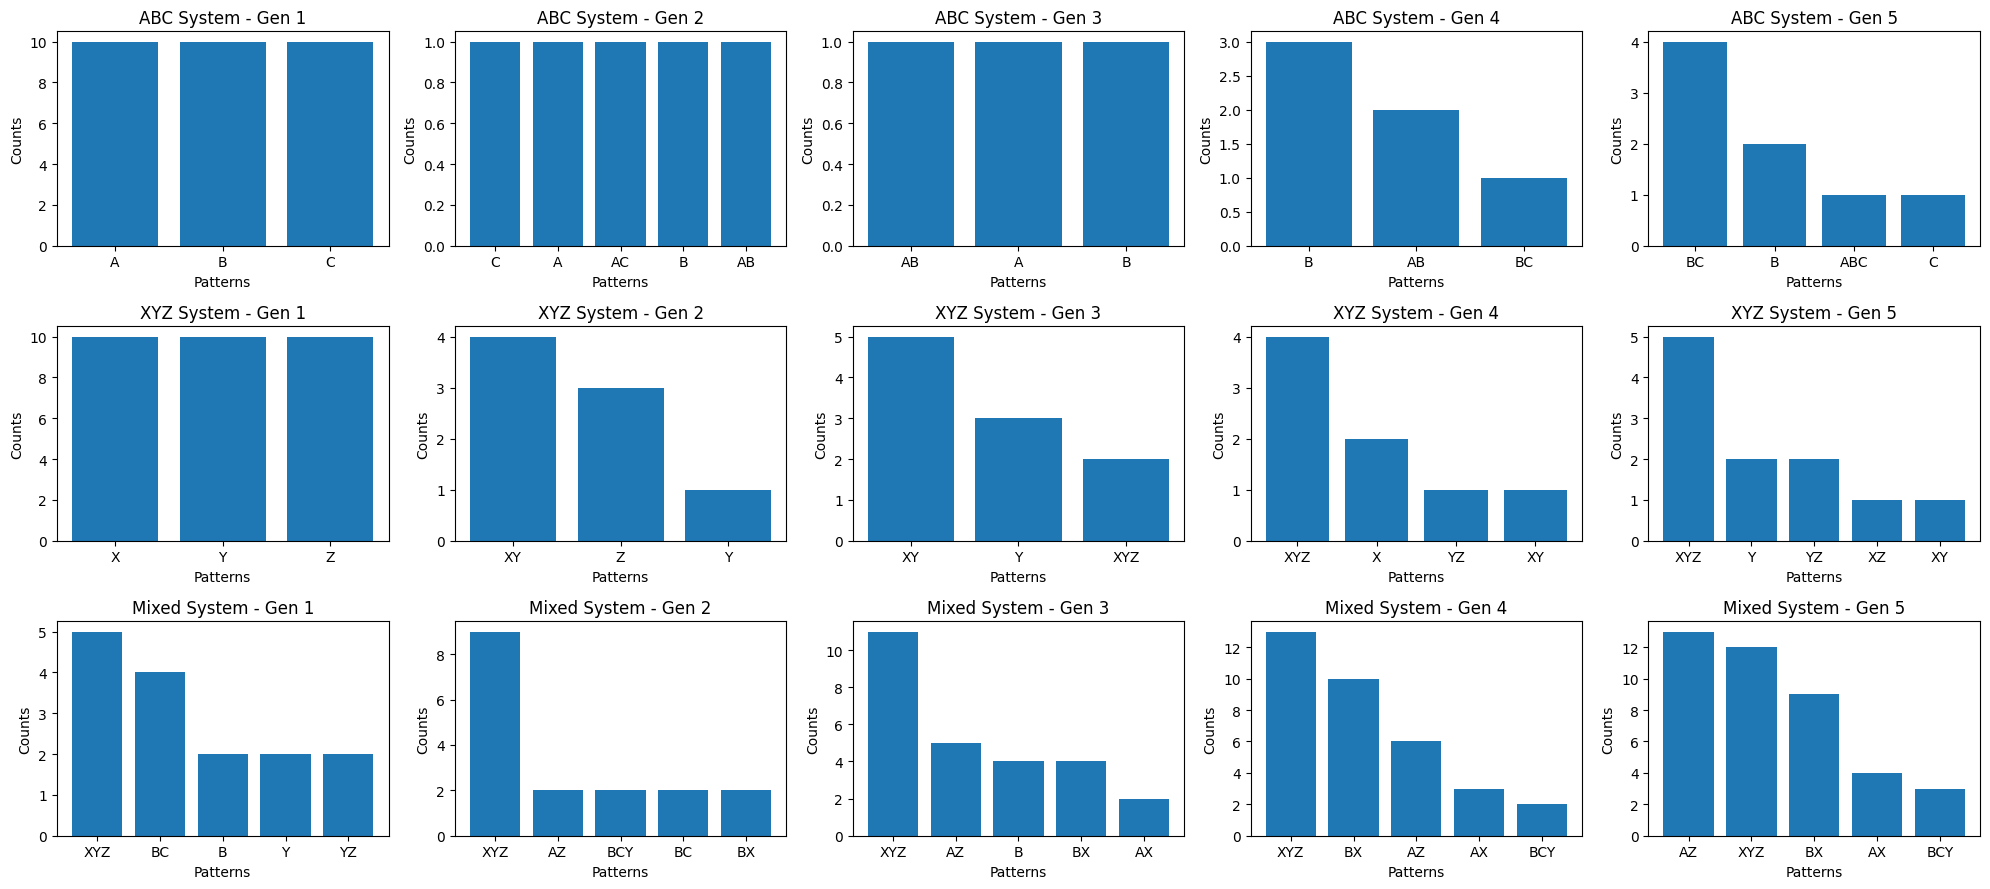
\includegraphics[width=13cm]{mixed_1}
    \caption{Mixing two evolved populations}
    \label{fig:mixed_1}
\end{figure}

\subsection{Entropy Dynamics in Mixed Systems}

After mixing, the joint entropy \( H_{\text{mix}}(t) \) becomes:
\[
H_{\text{mix}}(t) = -\sum_{p \in P_1 \cup P_2} P(p_t) \ln P(p_t),
\]
where \( P(p_t) \) now includes probabilities of cross-system patterns.

If both \( P_1 \) and \( P_2 \) are in low-entropy states, characterized by dominance of stable patterns, the mixed system is likely to retain a low entropy. The interaction of well-organized patterns results in selective formation of cross-system compounds, reinforcing order.

If either \( P_1 \) or \( P_2 \) has high entropy, the mixing introduces randomness into the more ordered system. Cross-system interactions may lead to transient increases in entropy, but selection pressures favoring stable compounds can gradually reduce entropy in subsequent generations.

When \( P_1 \) and \( P_2 \) have complementary patterns (e.g., \( P_1 \) lacks certain patterns that \( P_2 \) provides), mixing can generate new stable configurations that reduce entropy more effectively than in isolated systems. For instance, if \( P_1 = \{A, B\} \) and \( P_2 = \{X, Y\} \), the formation of \( ABX, BY, AX \) introduces novel low-entropy configurations.


\section{Interpreting Interactions as Logic Gates in ABC Systems}

ABC systems can be interpreted as encoding logical operations through their interactions, with patterns and their combinations acting as inputs and outputs of logical gates. Catalysis, a common feature in chemical systems, further reinforces this interpretation, as catalysts act as conditional enablers for specific reactions. This section explores how interactions in ABC systems can be mapped to logical operations and how catalytic behaviors correspond to logical gates or conditional statements.

\subsection{Interactions as Logical Operations}

In an ABC system, the combination of patterns can represent logical relationships. For instance, the interaction \( A + B \to AB \) can be interpreted as a logical AND operation, where \( AB \) is produced only if both \( A \) and \( B \) are present. The probabilities of patterns encode their logical "truth values," with higher probabilities corresponding to "true" states and lower probabilities corresponding to "false" states. We already showed that interaction \( A + B \to AB \) can be expressed as:
\[
P(AB) = P(A) \cdot P(B) \cdot S(AB),
\]
where \( S(AB) \) is the Stability. This is analogous to the AND operation in logic, where the output is true only if both inputs are true. Similarly, the OR operation can be represented as the dominance of either \( A \) or \( B \), given by:
\[
P(A \lor B) = P(A) + P(B) - P(A) \cdot P(B).
\]
The logical NOT operation corresponds to the absence of a pattern, represented as:
\[
P(\neg A) = 1 - P(A).
\]
These interactions collectively encode basic logical operations, enabling the system to process and store information in a manner analogous to digital logic.

\subsection{Catalysis as Conditional Logic}

In the context of ABC systems, a catalyst \( C \) facilitating the reaction \( A + B \to AB \) can be interpreted as a conditional statement or a logical gate. The presence of \( C \) determines whether the reaction occurs, making it analogous to the logical "if" condition: "If \( C \), then \( A + B \to AB \)."
This behavior maps directly to the conditional logic often found in programming and computation. In terms of probability, the catalyzed interaction can be expressed as:
\[
P(AB | C) \propto P(A) \cdot P(B) \cdot S(A, B | C),
\]
where \( S(A, B | C) \) represents the stability of the interaction in the presence of the catalyst \( C \).

Catalysts can also be compared to the gate of a transistor in an electronic circuit. Just as a transistor gate controls the flow of current between its source and drain, a catalyst \( C \) controls the occurrence of the reaction \( A + B \to AB \). The analogy extends to the amplification effect: a small amount of \( C \) can enable significant interaction between \( A \) and \( B \), similar to how a small gate voltage modulates a larger current.

Additionally, catalysts can encode more complex logical gates. For example, a two-step catalysis process \( C_1 \) and \( C_2 \) enabling \( A + B \to AB \) and \( AB + C \to ABC \) respectively corresponds to a sequential logic operation:
\[
\text{IF } C_1, \text{ THEN } A + B \to AB, \quad \text{AND IF } C_2, \text{ THEN } AB + C \to ABC.
\]
Such catalytic networks can encode conditional logic akin to nested IF statements in programming or complex gates in digital logic circuits. 

Interactions in ABC systems can be interpreted as logical operations, with catalysts playing the role of conditional gates or enabling mechanisms. This mapping reveals a computational aspect of such systems, where reactions and stability constraints naturally encode logic. Catalytic behaviors extend this logic by introducing conditionality, enabling ABC systems to perform more complex computations. These insights bridge the gap between chemical interactions and digital computation, highlighting the potential for emergent logic and information processing in abiotic systems.


\section{Generating Cellular Automata Rules in ABC Systems}

ABC systems, with their interaction-driven dynamics and stability-based selection, can be extended to generate behavior analogous to cellular automata (CA) \cite{wolfram2002new}. By carefully defining interaction rules and stability imbalances, ABC systems can mimic specific CA rules, including those capable of producing complex behavior. This section demonstrates how stability imbalances in an ABC system can emulate one of Wolfram’s elementary cellular automata rules and explores the mechanisms by which these systems transition into computational models.

\subsection{Mapping ABC Systems to Cellular Automata}

Cellular automata operate on discrete states, where the next state of a cell depends on its current state and the states of its neighbors. Similarly, ABC systems evolve based on the interactions and stabilities of patterns in the population. By associating patterns in the ABC system with the states of a CA, and interactions with transition rules, we can map ABC dynamics to CA behavior.

\subsection{Stability Imbalances as Transition Rules}

In ABC systems, the stability of interactions \( S(p, q) \) determines the likelihood of forming new patterns. To emulate a specific CA rule, we assign stability imbalances that prioritize the creation of patterns corresponding to the rule’s outputs. For instance, if the CA rule specifies that a cell becomes "active" when one or both neighbors are active, we increase the stability of interactions that encode this outcome.

Wolfram’s Rule 30 \cite{wolfram1983statistical} is a well-known elementary CA rule producing complex behavior. 
This can be encoded in an ABC system by associating the states of cells with patterns and defining stability imbalances to favor interactions that generate the correct next state. For example: we define \( A, B, C \) as the current states of left, center, and right cells, respectively. Then, use stability imbalances to prioritize outcomes matching the rule. For instance:
    \[
    S(A, B) = 0.9 \text{ if } A = 1, B = 1; \quad S(B, C) = 0.7 \text{ if } B = 1, C = 0.
    \]

We initialize the ABC system with patterns corresponding to the initial state of the CA and allow it to evolve according to the stability-driven dynamics. For example:
\begin{enumerate}
    \item Initialize the system with a random distribution of \( A, B, C \) (e.g., \( 101100110 \)).
    \item Define interaction rules such as \( A + B \to AB \), with stability imbalances reflecting Rule 30’s transition table.
    \item Allow the system to iterate, updating patterns based on the outcomes of interactions.
\end{enumerate}

At each iteration, the patterns \( AB, BC, \) etc., encode the next generation of the CA. The emergent dynamics will reflect the behavior of Rule 30, with complex patterns arising over successive generations.

\begin{figure}[htp]
    \centering
    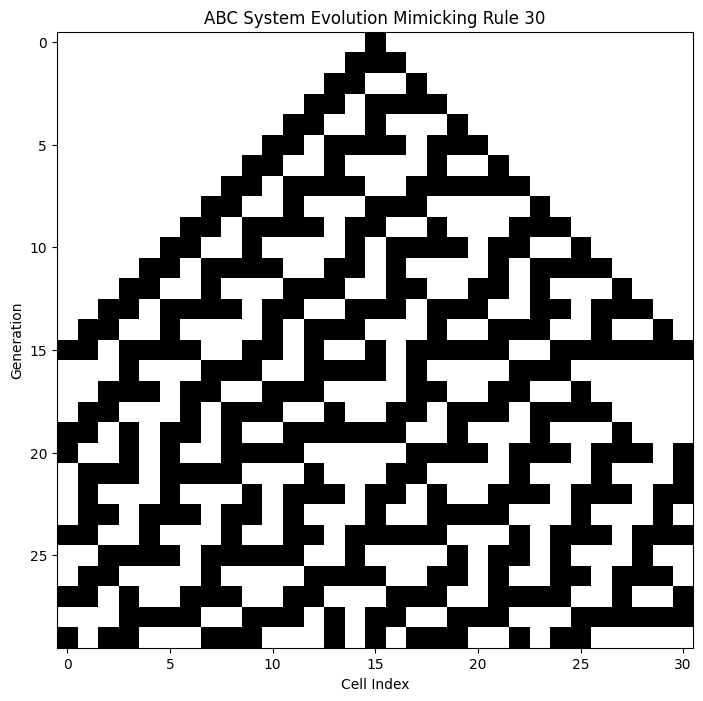
\includegraphics[width=8cm,height=6cm]{ca_1}
    \caption{ABC System Evolution Mimicking Rule 30}
    \label{fig:ca_1}
\end{figure}

The ability of ABC systems to replicate CA behavior highlights their potential for emergent computation and complex pattern formation.

\section{Fractals and Grid-Based Agent-Based Models in ABC Systems}

Fractals are mathematical structures characterized by self-similarity, where patterns repeat at different scales. Cellular automata (CA) have been widely used to generate fractals, such as the Sierpinski triangle, through simple, deterministic rules. ABC systems, however, offer a more generalized framework for simulating fractals and other grid-based phenomena by incorporating \textit{positional stability} and \textit{probabilistic evolution}. These enhancements extend the capabilities of ABC systems beyond deterministic CA, enabling the modeling of more dynamic and biologically inspired processes.

\subsection{Positional Stability in ABC Systems}

In traditional CA, the state of a cell depends solely on its current value and the values of its neighbors according to fixed transition rules. In ABC systems, the concept of \textit{positional stability} allows the interactions between elements to depend on both the spatial relationships and the inherent stabilities of those interactions. Specifically, the likelihood of a cell transitioning to a specific state is determined by stability scores assigned to its neighbors' positions, such as \textit{left}, \textit{center}, and \textit{right}. This approach mimics chemical bonding, where interactions may vary depending on direction and context.

For instance, in a grid-based ABC system designed to generate fractal patterns:
\[
S(\text{left}), S(\text{center}), S(\text{right})
\]
represent the stability scores of interactions for each position in a triplet. The system evolves probabilistically, with the stability scores determining the likelihood of an element transitioning to an active (\textit{e.g.,} `A') or inactive (\textit{e.g.,} `B') state. Additionally, a small mutation rate introduces stochasticity, ensuring the exploration of a broader pattern space.

\subsection{Simulating the Sierpinski Triangle with Positional Stability}

Using positional stability, an ABC system can simulate patterns resembling fractals, such as the Sierpinski triangle. Figure~\ref{fig:fractals} illustrates the comparison between the classic Sierpinski triangle generated using deterministic CA rules and the emergent pattern from an ABC system incorporating probabilistic, stability-driven dynamics. While the simulated pattern does not perfectly match the mathematical Sierpinski triangle, it demonstrates the capacity of ABC systems to approximate fractal-like behavior using generalized, probabilistic rules.

\begin{figure}[ht]
    \centering
    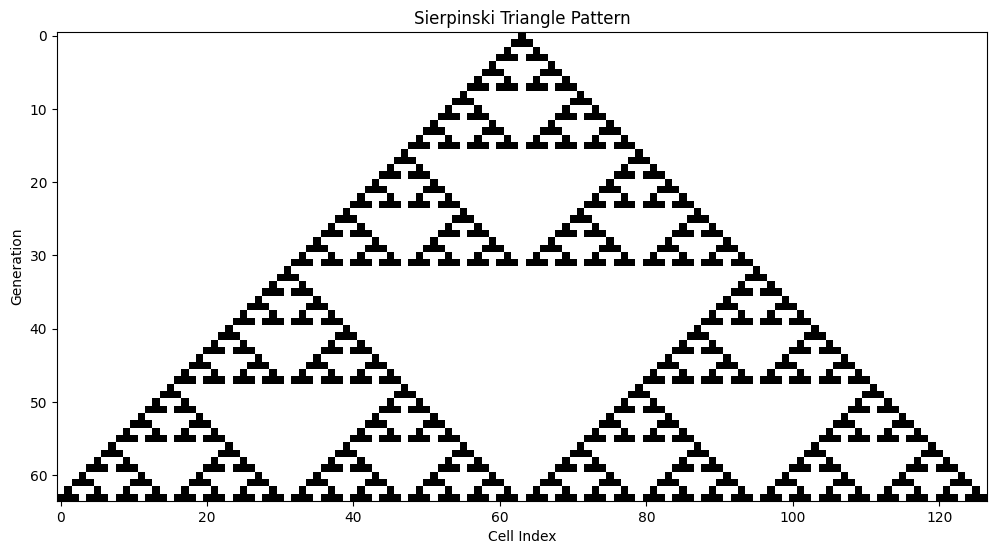
\includegraphics[width=0.45\textwidth]{sierpinski_actual.png}
    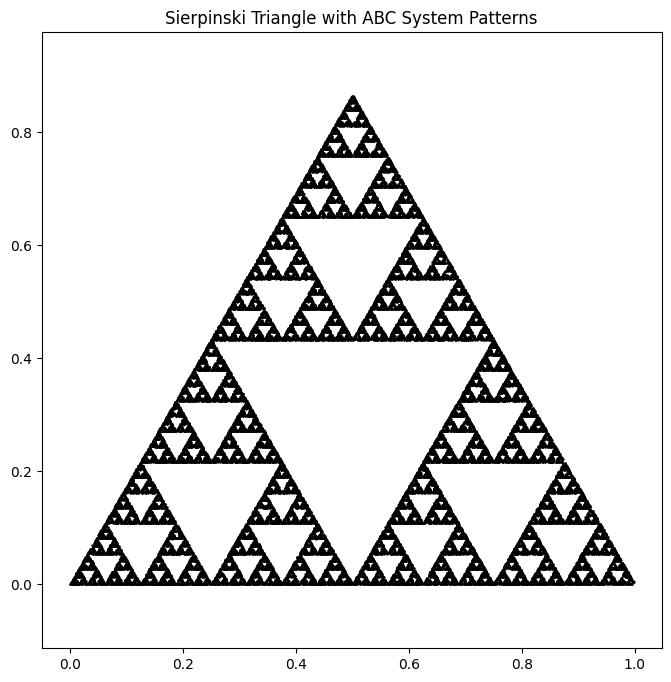
\includegraphics[width=0.45\textwidth]{sierpinski_simulated.png}
    \caption{Left: Classic Sierpinski triangle generated by deterministic CA rules. Right: Emergent fractal-like pattern from an ABC system with positional stability.}
    \label{fig:fractals}
\end{figure}


\section{Bayesian Updating in ABC Systems}

ABC systems highlight a key distinction between Bayesian \cite{mcgrayne2011theory} updating and frequentist probabilities, illustrating their respective roles in evolving versus static systems. Bayesian updating provides a dynamic framework for incorporating new information over time, making it a hallmark of systems capable of evolution and self-organization. Frequentist probabilities, on the other hand, describe point-in-time static distributions, lacking the temporal adaptability intrinsic to evolutionary dynamics.

Kauffman \cite{kauffman2000investigations}, for example, has used frequentist arguments to claim that a purely computational system cannot explore the "adjacent possible". In ABC systems, the "adjacent possible" means compounds that emerge in generation \(t+1\), but were not available in generation \(t\). Thinking about the problem in Bayesian terms, removes his objection.

In ABC systems, the probability of a pattern \( p \) at generation \( t+1 \) depends on its prior probability \( P(p_t) \), the probabilities of other patterns \( P(q_t) \), and the stability of their interactions \( S(p, q) \). The update rule can be expressed as:
\[
P(p_{t+1}) = \frac{P(p_t) \cdot \sum_{q \in P} P(q_t) \cdot S(p, q)}{\sum_{p' \in P} P(p'_t) \cdot \sum_{q \in P} P(q_t) \cdot S(p', q)},
\]
where the numerator reflects the likelihood of \( p \) persisting or forming through interactions, and the denominator ensures normalization of probabilities. This is analogous to the Bayesian formula:
\[
P(H|E) = \frac{P(E|H) \cdot P(H)}{P(E)},
\]
where:
\begin{itemize}
    \item \( H \): Hypothesis (\( p \) as a pattern in the system).
    \item \( E \): Evidence (interactions \( q \) and their stabilities \( S(p, q) \)).
    \item \( P(H) \): Prior probability (\( P(p_t) \)).
    \item \( P(E|H) \): Likelihood (\( \sum_{q \in P} P(q_t) \cdot S(p, q) \)).
    \item \( P(H|E) \): Posterior probability (\( P(p_{t+1}) \)).
\end{itemize}

This iterative Bayesian updating process allows ABC systems to adapt and encode new information dynamically. The system continuously adjusts pattern probabilities to reflect the effects of interactions and stability constraints, resulting in emergent complexity and self-organization.

\section{Emergent Information vs. Pre-Designed Information in ABC Systems}

Emergent information arises from the interactions and feedback loops within a system. In ABC systems, patterns evolve dynamically as stable configurations persist and dominate over time through iterative interactions, encoding the history of the system. Selection pressure, driven by stability imbalances and probabilistic feedback, ensures that only certain configurations persist. This process guides the system toward lower-entropy, information-rich states. Unlike systems with predetermined outcomes, ABC systems explore a vast configuration space, with the resulting patterns shaped by initial conditions, interaction rules, and stability constraints.

In contrast to ABC systems, pre-designed systems, such as 3D-printed compounds or pre-programmed circuits, rely on external means to define their structure and function. In such systems, information is imposed externally, with patterns explicitly specified by a designer or blueprint, leaving little or no room for system dynamics. These systems lack an evolutionary process and do not explore configuration space; instead, they are constructed to achieve predefined states. Consequently, their outcomes are fixed and static, with minimal capacity for adaptation or self-organization. The absence of emergent dynamics distinguishes these systems from the adaptable and exploratory nature of ABC systems.

The contrast between emergent and pre-designed systems suggests a potential criterion for determining whether a system is pre-designed: the presence of an evolutionary process. If a system displays emergent properties such as adaptation, path dependency, and entropy reduction, it likely evolves internally. Conversely, systems that achieve order without intermediate steps or feedback are more likely to be pre-designed. Machine learning systems lie on a continuum between pre-designed systems and fully emergent ones, since evolution-like processes occur under strong external guidance and predefined constraints.


\section{The Path from Abiotic to Biotic Evolution in ABC Systems}

ABC systems offer a framework for understanding how evolutionary processes can emerge in abiotic contexts, bridging the gap between non-living matter and life-like behavior. By encoding memory, leveraging feedback, and fostering self-organization, these systems demonstrate that evolution arises from fundamental principles of stability and selection rather than being confined to living systems.

Abiotic evolution in ABC systems is driven by stability imbalances, interaction probabilities, and selection pressures. Stable patterns persist across generations, encoding information about the system’s history. This process mirrors natural selection, with stability acting as a fitness criterion. Over time, feedback loops amplify self-replicating patterns, creating networks of interactions that drive the emergence of increasingly complex and self-sustaining structures.

As stable patterns encode information and adapt dynamically, ABC systems act as rudimentary computational models, mimicking logic gates and cellular automata. The transition to biotic evolution occurs when these information-processing capabilities enable patterns to replicate and adapt more robustly, aligning with principles of Turing machines.

ABC systems highlight how evolutionary processes, including inheritance, metabolism, and selection, can emerge without predefined biological structures. By evolving information storage and self-replication, these systems offer a plausible pathway for abiotic systems to transition toward biotic behavior, providing insights into the origins of life and the emergence of complexity in non-living systems.


\section{Top-Down vs. Bottom-Up Dynamics in ABC Systems}

ABC systems provide a unique framework for exploring the interplay between top-down and bottom-up causality. In traditional systems, top-down causality refers to higher-level structures that govern individual components, while bottom-up causality arises from local interactions that collectively create emergent behavior. In ABC systems, both forms of causality co-exist, enabling the study of their co-dependence in generating complexity.

Bottom-up causality is evident in the formation of patterns through probabilistic interactions and selection pressures. Local rules, such as compound stability or reaction probabilities, drive the evolution of patterns, creating stability and reducing entropy. Simultaneously, top-down causality manifests in feedback loops, where stable patterns persisting across generations influence future interactions. For instance, a dominant compound like \( AB \) biases subsequent interactions, catalyzing the formation of related patterns and introducing a higher-level influence over bottom-up processes.

This co-dependence suggests that neither top-down nor bottom-up dynamics alone can explain complexity. ABC systems highlight how emergent patterns dynamically impose top-down constraints, which in turn stabilize and refine bottom-up processes. By abstracting specific physical laws, ABC systems offer a generalizable model for causality in complex systems, bridging abiotic and biotic evolution. This perspective has broad implications for understanding the emergence of order and information across natural and computational systems.


%\begin{listing}[H]
%\caption{Title of the listing}
%\rule{\columnwidth}{1pt}
%\raggedright Text of the listing. In font size footnotesize, small, or normalsize. Preferred format: left aligned and single spaced. Preferred border format: top border line and bottom border line.
%\rule{\columnwidth}{1pt}
%\end{listing}

%%%%%%%%%%%%%%%%%%%%%%%%%%%%%%%%%%%%%%%%%%
\vspace{6pt} 

%%%%%%%%%%%%%%%%%%%%%%%%%%%%%%%%%%%%%%%%%%
%% optional
%\supplementary{The following supporting information can be downloaded at:  \linksupplementary{s1}, Figure S1: title; Table S1: title; Video S1: title.}

% Only for journal Methods and Protocols:
% If you wish to submit a video article, please do so with any other supplementary material.
% \supplementary{The following supporting information can be downloaded at: \linksupplementary{s1}, Figure S1: title; Table S1: title; Video S1: title. A supporting video article is available at doi: link.}

% Only for journal Hardware:
% If you wish to submit a video article, please do so with any other supplementary material.
% \supplementary{The following supporting information can be downloaded at: \linksupplementary{s1}, Figure S1: title; Table S1: title; Video S1: title.\vspace{6pt}\\
%\begin{tabularx}{\textwidth}{lll}
%\toprule
%\textbf{Name} & \textbf{Type} & \textbf{Description} \\
%\midrule
%S1 & Python script (.py) & Script of python source code used in XX \\
%S2 & Text (.txt) & Script of modelling code used to make Figure X \\
%S3 & Text (.txt) & Raw data from experiment X \\
%S4 & Video (.mp4) & Video demonstrating the hardware in use \\
%... & ... & ... \\
%\bottomrule
%\end{tabularx}
%}

%%%%%%%%%%%%%%%%%%%%%%%%%%%%%%%%%%%%%%%%%%

\funding{This research received no external funding}

\institutionalreview{Not applicable}

\informedconsent{Not applicable}

\dataavailability{Not applicable} 

\acknowledgments{}

\conflictsofinterest{The author declares no conflicts of interest} 

%%%%%%%%%%%%%%%%%%%%%%%%%%%%%%%%%%%%%%%%%%
%%%%%%%%%%%%%%%%%%%%%%%%%%%%%%%%%%%%%%%%%%
%%%%%%%%%%%%%%%%%%%%%%%%%%%%%%%%%%%%%%%%%%
\begin{adjustwidth}{-\extralength}{0cm}
%\printendnotes[custom] % Un-comment to print a list of endnotes

\reftitle{References}

% Please provide either the correct journal abbreviation (e.g. according to the “List of Title Word Abbreviations” http://www.issn.org/services/online-services/access-to-the-ltwa/) or the full name of the journal.
% Citations and References in Supplementary files are permitted provided that they also appear in the reference list here. 

%=====================================
% References, variant A: external bibliography
%=====================================
%\bibliography{your_external_BibTeX_file}

%=====================================
% References, variant B: internal bibliography
%=====================================
\begin{thebibliography}{999}
\bibitem{schrodinger1944life}
Schrödinger, E. \textit{What is Life?}; Cambridge University Press: Cambridge, UK, 1944.

\bibitem{tegmark2008mathematical}
Tegmark, M. The Mathematical Universe. \textit{Found. Phys.} \textbf{2008}, \textit{38}, 101–150. https://doi.org/10.1007/s10701-007-9186-9.

\bibitem{nowak2006evolutionary}
Nowak, M.A. \textit{Evolutionary Dynamics: Exploring the Equations of Life}; Belknap Press: Cambridge, MA, USA, 2006.

\bibitem{wheeler1990itbit}
Wheeler, J.A. Information, Physics, Quantum: The Search for Links. In \textit{Complexity, Entropy, and the Physics of Information}; Zurek, W.H., Ed.; Addison-Wesley: Redwood City, CA, USA, 1990; pp. 3–28.

\bibitem{noble2012causality}
Noble, D. A Theory of Biological Relativity: No Privileged Level of Causation. \textit{Interface Focus} \textbf{2012}, \textit{2}, 55–64. https://doi.org/10.1098/rsfs.2011.0067.

\bibitem{lloyd2006programming}
Lloyd, S. \textit{Programming the Universe: A Quantum Computer Scientist Takes on the Cosmos}; Alfred A. Knopf: New York, NY, USA, 2006.

\bibitem{kolmogorov1965complexity}
Kolmogorov, A.N. Three Approaches to the Quantitative Definition of Information. \textit{Problemy Peredachi Informatsii} \textbf{1965}, \textit{1}, 3–11.

\bibitem{chaitin1977algorithmic}
Chaitin, G.J. Algorithmic Information Theory. \textit{IBM J. Res. Dev.} \textbf{1977}, \textit{21}, 350–359. https://doi.org/10.1147/rd.215.0350.

\bibitem{solomonoff1964formal}
Solomonoff, R.J. A Formal Theory of Inductive Inference. Part I and Part II. \textit{Inf. Control} \textbf{1964}, \textit{7}, 1–22, 224–254. https://doi.org/10.1016/S0019-9958(64)90223-2.


\bibitem{shannon1948mathematical}
Shannon, C.E. A Mathematical Theory of Communication. \textit{Bell Syst. Tech. J.} \textbf{1948}, \textit{27}, 379–423. https://doi.org/10.1002/j.1538-7305.1948.tb01338.x.

\bibitem{back1996evolutionary}
Bäck, T.; Fogel, D.B.; Michalewicz, Z. \textit{Evolutionary Computation 1: Basic Algorithms and Operators}; CRC Press: Boca Raton, FL, USA, 2000.

\bibitem{goldberg1989genetic}
Goldberg, D.E. \textit{Genetic Algorithms in Search, Optimization, and Machine Learning}; Addison-Wesley: Boston, MA, USA, 1989.

\bibitem{holland1975adaptation}
Holland, J.H. \textit{Adaptation in Natural and Artificial Systems}; University of Michigan Press: Ann Arbor, MI, USA, 1975.

\bibitem{leff2002maxwell}
Leff, H.S.; Rex, A.F. \textit{Maxwell’s Demon: Entropy, Information, Computing}; Princeton University Press: Princeton, NJ, USA, 2002.

\bibitem{wolfram1983statistical}
Wolfram, S. Statistical Mechanics of Cellular Automata. \textit{Rev. Mod. Phys.} \textbf{1983}, \textit{55}, 601–644. https://doi.org/10.1103/RevModPhys.55.601.

\bibitem{wolfram2002new}
Wolfram, S. \textit{A New Kind of Science}; Wolfram Media: Champaign, IL, USA, 2002.

\bibitem{mcgrayne2011theory}
McGrayne, S.B. \textit{The Theory That Would Not Die: How Bayes' Rule Cracked the Enigma Code, Hunted Down Russian Submarines, and Emerged Triumphant from Two Centuries of Controversy}; Yale University Press: New Haven, CT, USA, 2011.

\bibitem{kauffman2000investigations}
Kauffman, S. \textit{Investigations}; Oxford University Press: New York, NY, USA, 2000.

\end{thebibliography}

% If authors have biography, please use the format below
%\section*{Short Biography of Authors}
%\bio
%{\raisebox{-0.35cm}{\includegraphics[width=3.5cm,height=5.3cm,clip,keepaspectratio]{Definitions/author1.pdf}}}
%{\textbf{Firstname Lastname} Biography of first author}
%
%\bio
%{\raisebox{-0.35cm}{\includegraphics[width=3.5cm,height=5.3cm,clip,keepaspectratio]{Definitions/author2.jpg}}}
%{\textbf{Firstname Lastname} Biography of second author}

% For the MDPI journals use author-date citation, please follow the formatting guidelines on http://www.mdpi.com/authors/references
% To cite two works by the same author: \citeauthor{ref-journal-1a} (\citeyear{ref-journal-1a}, \citeyear{ref-journal-1b}). This produces: Whittaker (1967, 1975)
% To cite two works by the same author with specific pages: \citeauthor{ref-journal-3a} (\citeyear{ref-journal-3a}, p. 328; \citeyear{ref-journal-3b}, p.475). This produces: Wong (1999, p. 328; 2000, p. 475)

%%%%%%%%%%%%%%%%%%%%%%%%%%%%%%%%%%%%%%%%%%
%% for journal Sci
%\reviewreports{\\
%Reviewer 1 comments and authors’ response\\
%Reviewer 2 comments and authors’ response\\
%Reviewer 3 comments and authors’ response
%}
%%%%%%%%%%%%%%%%%%%%%%%%%%%%%%%%%%%%%%%%%%
\PublishersNote{}
\end{adjustwidth}
\end{document}

